\section{A non-technical overview}\label{sec:overview}
This section explains the setting and the main statements without
technical prerequisites. Figure~\ref{fig:overview} summarizes it in one
picture. The precise statements, their evidence and their limits are
those of the later sections; nothing here adds a result.

\paragraph{What is a Q-ball?}
A Q-ball is a lump of a field that holds itself together. The field in
this paper is a complex scalar field, a quantity with a size and an
internal phase at every point of space. In a Q-ball the size forms a
round, localized profile, while the internal phase turns steadily in
time, like the hand of a clock with angular frequency~$\omega$. The
density of the field, and therefore the shape of the lump, does not
change in time (Fig.~\ref{fig:overview}a). The rotation carries a
conserved charge~$Q$, which plays the role of a particle number.
Coleman showed that, in suitable theories with such a conserved charge,
lumps of sufficiently large charge have less energy than the same charge
carried by free particles; such lumps cannot simply fall apart and are
stable~\cite{Coleman1985}. This general argument concerns large charge;
the stability of the particular backgrounds of this paper is not
established here. Friedberg, Lee and Sirlin had earlier constructed related
nontopological solitons, which also rely on a conserved additive quantum
number, in a model with an additional neutral
field~\cite{FriedbergLeeSirlin1976}. Q-balls with a large charge have a
nearly uniform interior and a transition zone of fixed thickness at the
surface~\cite{Coleman1985}. In the present model this thin-wall regime
is reached as $\omega^2$ approaches $1/2$; the wall keeps its thickness
while the radius grows, so the wall becomes thin relative to the ball.

\paragraph{What holds it together?}
The shape follows from a balance of competing tendencies. Gradients cost
energy, so the field profile is smoothed and any edge is softened. Far
outside, the field decays to zero because of its mass and because
$\omega^2<1$. The potential $\mathcal U(S)=S-S^2+S^3/2$ of the field
density $S=|\phi|^2$ contains a negative term $-S^2$, which lowers the
energy relative to free, non-interacting field, and a positive term
$S^3/2$, which penalizes high density. At fixed conserved charge this
combination permits binding; in the thin-wall regime the preferred
interior density tends to $S=1$. Coleman gave an intuitive picture of
this balance~\cite{Coleman1985}: the equation for the radial profile is
the equation of motion of a particle whose position is the field value
and whose time is the radius. The particle moves in a landscape with two
hills and is slowed by a damping term that becomes weaker at large
radius (Fig.~\ref{fig:overview}b). A Q-ball corresponds to a particle
that starts at rest on the inner side of the outer hill and comes to
rest exactly on the hill at zero field. For the present potential this
is possible only for $1/2<\omega^2<1$. Close to $\omega^2=1/2$ the two
hills have almost equal height; the particle then starts very close to
the top and lingers there, which gives a large uniform core with a
comparatively thin wall.

\paragraph{Vibrations, two channels and radiation.}
A Q-ball can vibrate. A small vibration with frequency $\rho$ of the
rotating lump appears in the field at two partner frequencies,
$\omega+\rho$ and $\omega-\rho$; these coupled sidebands are the standard
description of Q-ball perturbations~\cite{Kovtun2018}. Far from the
ball, a component can travel outwards as a wave only if the magnitude of
its frequency exceeds one, the mass of the field in our units; below
that threshold its tail decays exponentially. A negative frequency, as
for $\omega-\rho$ here, only means that the phase turns the other way.
In the regime studied here one partner lies above the threshold and the
other below it (Fig.~\ref{fig:overview}c). The upper partner is an open
channel: it can carry energy away to infinity as radiation. The lower
partner is a closed channel: it is trapped near the ball. Excited
Q-balls have vibrational modes~\cite{Kovtun2018}, and in a
one-dimensional version of the same type of model a squashed Q-ball
relaxes by radiating through such channels~\cite{Ciurla2024}. A typical
vibration in our regime should therefore leak energy and fade. Its
leakage rate is measured by the width of the resonance: the larger the
width, the faster the vibration fades.

\paragraph{When the radiation vanishes.}
How much energy leaks depends on the amplitude of the outgoing wave in
the open channel. Contributions to this wave from different parts of
the ball can cancel each other by interference. When they cancel
completely, the width is zero and the vibration stays exactly localized
although a radiation channel is open. Such a state is a bound state in
the continuum (BIC): a localized wave that coexists with extended waves
of the same frequency but does not radiate~\cite{Hsu2016}. The idea was
proposed in quantum mechanics as early as 1929 by von Neumann and
Wigner, and BICs have since been studied in many wave systems,
particularly in photonics; one known route is the cancellation of
radiating components, for example when two interacting resonances
interfere so that the width of one of them
vanishes~\cite{Hsu2016,FriedrichWintgen1985}.
Figure~\ref{fig:overview}d shows the computed mode C0: its open-channel
component decays like the trapped one instead of leaving an outgoing
tail.

\paragraph{Why this is not automatic.}
Three reasons make such cancellations nontrivial. First, once the
background and the overall size of the vibration are fixed, the outgoing
wave must vanish in both of its oscillation phases. These are two real
matching conditions for the two frequencies $\omega$ and $\rho$.
Generically this suggests that cancellations, if they occur, sit at
isolated parameter points that have to be found. The proofs below
establish existence inside small parameter boxes; they do not establish
that the parameter pair is unique. Second, for a single wave scattered
by an object of finite extent, such trapped states are generally
excluded~\cite{Hsu2016}. The Q-ball problem is of a different kind: the
vibration has two coupled components, one of which cannot propagate.
For the linearization about the ground state of the focusing cubic
nonlinear Schr\"odinger equation in three dimensions, embedded
eigenvalues are proved to be absent~\cite{LiYang2026}; the present
relativistic model is different, and nothing here contradicts that
theorem. Third, a computer calculation in a finite box can show a very
small width that is not exactly zero. Only a proof that controls the
infinite exterior separates an exact zero from a near miss. This is the
reason for the computer-assisted proofs in
Section~\ref{sec:certified-existence}. They use interval arithmetic,
which carries guaranteed bounds through every rounded arithmetic
operation, together with analytic estimates that bound the remaining
approximation errors and the infinite exterior.

\paragraph{Proved cancellations and numerical candidates.}
Figure~\ref{fig:overview}e and Fig.~\ref{fig:ladder} show where
cancellations of the spherically symmetric vibrations have been proved
or numerically located. Eighteen locations are reported, labelled
$n=1,\ldots,18$; they move from $\omega^2\approx0.798$ towards the
thin-wall threshold $\omega^2=1/2$. Only the first two, C0 and C1, are
exact zeros established by computer-assisted proofs with analytic control
of the infinite exterior. A third proof, C2, concerns a dipole vibration,
in which two opposite halves of the ball oscillate against each other;
it belongs to a separate angular channel. The other sixteen locations
are numerical candidates, for which an exact zero is not established,
with the graded evidence of Table~\ref{tab:ladder}. For $n=3$--$15$ a
numerical winding test was resolved: the two matching errors were seen
to circle zero once around the candidate (for $n=5$ and $11$--$14$ in a
calculation added in this revision), and $n=16$--$18$ failed the final
acceptance rule. Figure~\ref{fig:overview}e still marks $n=5$ and
$11$--$14$ with the weaker evidence classes of preprint 0.52; their
location changes are below its plotting resolution. The inverse detuning $1/(\omega^2-1/2)$ measures how
close a ball is to the thin-wall threshold. Plotted against it, the
locations are nearly equally spaced; between indices 12 and 15 the steps
are about $2.30$ to $2.31$. In the thin-wall picture this has a simple
reading. The radius of the ball grows in proportion to the inverse
detuning, Eq.~\eqref{eq:thinwall}. The interior acts like a resonator
between the centre and the reflecting wall, and a further cancellation
appears whenever one more half wavelength fits into the interior
(Section~\ref{sec:thinwall}). This finite-radius phase description is
partly calibrated to the numerical results. If the interior wavelength
and the phase at the wall approach limits, it suggests approximately
equal steps; it is not a parameter-free prediction of all locations.
A separate calculation for a flat wall, not fitted to the locations,
gives a candidate value $2.3100$ for the step.

Several things are not shown. There is no proof of an infinite
ladder, and the identification of the flat-wall value with the actual
limiting step remains open; a frozen formula for the absolute locations
failed its test. The stability of the Q-ball backgrounds themselves is
not established. A numerical check of how the charge changes with the
frequency bears, under the assumptions of a standard criterion, only on
one simple kind of instability, a purely growing radial deformation, and
finds no sign of it (Section~\ref{sec:discussion}). Finally, the cancellation is a statement about small,
linear vibrations. At finite amplitude, nonlinear terms can drive second
harmonics, with laboratory frequencies $\omega\pm2\rho$; for the
certified modes these lie in the propagating range, but this alone does
not establish outgoing radiation. For the dipole mode C2, under stated
hypotheses, one outgoing second-harmonic coefficient is guaranteed to be
nonzero. This obstructs a specified smooth localized continuation to
finite amplitude, while circular polarization needs a separate
certificate (Section~\ref{nl:section}). For C1 the corresponding
calculation is open. The linear trapping found here therefore does not
establish a nonlinear trapping, and no lifetime or instability is
inferred.

\paragraph{Potential significance.}
The following points are possibilities for further work, not claims of
this paper. Numerical simulations indicate that Q-balls can form in
the early universe through the fragmentation of an Affleck--Dine scalar
condensate~\cite{KasuyaKawasaki2000}, and supersymmetric Q-balls have
been proposed as a contribution to dark
matter~\cite{KusenkoShaposhnikov1998}. Whether comparable linear
cancellations occur in such models, and whether they matter for how
long internal vibrations last, are open questions; the present model,
its parameters and the nonlinear limitation noted above support no
statement about lifetimes or observations. In photonics, BICs underlie
sharp resonances with high quality factors; in real structures of
finite size they appear as quasi-BICs, weakly leaking approximations to
an ideal BIC~\cite{Koshelev2018}, with applications ranging from lasers
and sensors to filters~\cite{Hsu2016}. The Q-ball zeros share the
interference and resonator logic of such systems; this is an analogy of
mechanism, and no experimental realization is proposed. Finally, the
combination of interval arithmetic with analytic control of the
infinite exterior used here is a general method: it can separate exact
embedded eigenvalues from small numerical widths in other soliton
problems, in the spirit of related computer-assisted spectral
work~\cite{LuhrmannEtAl2026,MarzuolaSimpson2011}. None of this amounts
to a stability result, a particle model or an experimental proposal.

\begin{figure}[p]\centering
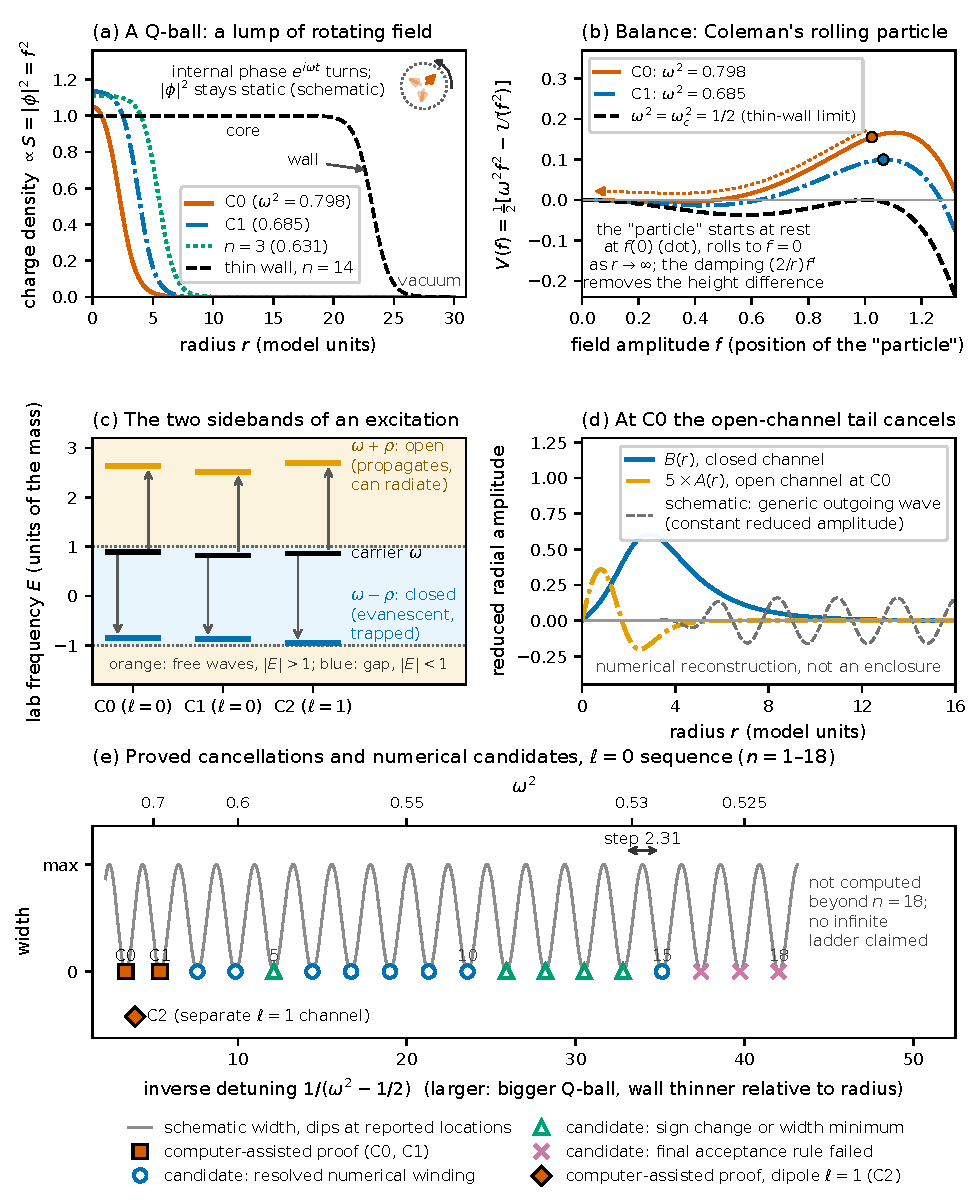
\includegraphics[width=.95\linewidth]{qball-overview.pdf}
\caption{Overview of the objects studied in this paper.
(a)~Density profiles $S=f^2$ of stored backgrounds (C0, C1, $n=3$) and
the leading thin-wall formula, Eq.~\eqref{eq:thinwall}, at the
$\omega^2$ of index $14$; the inset is schematic.
(b)~Coleman's mechanical picture of Eq.~\eqref{eq:profile}~\cite{Coleman1985}
with $V(f)=\frac12[\omega^2f^2-\mathcal U(f^2)]$; dots mark the stored
central values $f(0)$.
(c)~Sideband frequencies $\omega\pm\rho$ of the three certified modes
(Table~\ref{tab:proof-cases}) relative to the threshold $|E|=1$ of
Eq.~\eqref{eq:channels}.
(d)~Stored numerical reconstruction of the C0 channel functions, not a
pointwise enclosure. $A=ra$ and $B=rb$ remove the $1/r$ spreading, so
the schematic outgoing wave has constant reduced amplitude while its
physical field falls as $1/r$.
(e)~Locations of Table~\ref{tab:ladder} and of C2 on the inverse-detuning
axis, marked by evidence class (preprint 0.52). The grey width curve is schematic: its
dips are placed at the reported locations, and a zero depth is
established only for C0, C1 and C2. The step label is the difference
between indices 14 and 15; nothing beyond $n=18$ is computed or implied.
Sources and checksums: Section~\ref{app:provenance}.}
\label{fig:overview}
\end{figure}
